\documentclass[12pt]{article}
\usepackage[margin=1in]{geometry}

\usepackage[T1]{fontenc}
\usepackage[utf8]{inputenc}
\usepackage[english,polish]{babel}
\selectlanguage{polish}
\usepackage{lmodern}

\usepackage{tabularx}
\usepackage{graphicx}
\usepackage{enumitem}
\usepackage{tikz}
\usepackage{color}
\usetikzlibrary{decorations.markings}

\newcommand*\raiseedge{{\scriptsize\tikz[scale = 0.4, baseline=(b.base), >=stealth]{
      \draw[-,postaction={decoration={markings,mark=at position 0.6 with {\arrow{>}}},decorate}
      ] (0, 0) node(b){} -- ++(0:1) -- ++(80:1) -- ++(0:1);}}}

\begin{document}
\newcolumntype{C}[1]{>{\centering\arraybackslash}p{#1}}

\title{Akademia ETI\\\large Instrukcja do laboratorium}
\author{Jan Olencki, Jakub Gierowski,\\Mikołaj Barcikowski, Maciej Brzeski}
\date{27 lutego 2019}
\maketitle
\textbf{\textcolor{red}{Uwaga! Wszelkie nazwy utworzonych plików lub folderów nie mogą zawierać polskich znaków!\\
Przed utworzeniem nowego projektu należy zamknąć poprzedni (File > Close project)!}}
\section{Przerzutnik typu JK}
\begin{table}[h!]
\renewcommand{\arraystretch}{1.5}
\begin{center}
\begin{tabular}{|C{0.4in}|C{0.4in}|C{0.4in}|C{0.4in}|C{0.4in}|}
\hline
\hline
$CLK$ & $J$ & $K$ & $Q_{t+1}$ & $\overline{Q_{t+1}}$	\\
\hline
\raiseedge & 0 & 0 & $Q_{t}$ & $\overline{Q_{t}}$ \\
\raiseedge & 0 & 1 & 0 & 1 \\
\raiseedge & 1 & 0 & 1 & 0 \\
\raiseedge & 1 & 1 & $\overline{Q_{t}}$ & $Q_{t}$ \\
\hline
\hline
\end{tabular}
\caption{Tabela wzbudzeń przerzutnika typu JK.}
\label{tab:table1}
\end{center}
\renewcommand{\arraystretch}{1}
\end{table}
Tablica prawdy pokazuje, jaka wartość będzie na wyjsciu przerzutnika(Q) w zalezności od jego wejść J i K oraz sygnału zegarowego CLK. Wartość 1 oznacza stan wysoki, a wartość 0 stan niski. Przerzutnik pracuje w takt zegara, kiedy zmienia się zbocze sygnału zegarowego, czyli kiedy wartość zmienia się z 0 na 1.
\subsection{Do wykonania}
\begin{enumerate}[wide, labelwidth=!, labelindent=0pt]
\item Utworzyć nowy projekt w programie Xilinx~ISE~10.1 i dodać do niego odpowiednie pliki źródłowe.
\item Przeanalizować schemat układu. Jaką częstotliwością taktowany jest układ przerzutnika? Które przyciski odpowiadają sygnałom J i K? Jak zostanie wyświetlony sygnał Q?
\item Przeprowadzić symulację układu.
\item Wgrać program do systemu docelowego. Co się dzieje gdy oba przyciski J i K są wciśnięte?
\end{enumerate}
\subsection{Krok po kroku}
\begin{enumerate}[wide, labelwidth=!, labelindent=0pt]
\item Ze strony pobrać folder \textit{jk\_flip\_flop}.
\item Należy uruchomić program Xilinx ISE 10.1
\item Utworzyć nowy projekt poprzez File > New Project.
Upewnić się, że został wybrany folder taki jak na rysunku. Podać nazwę projektu i wybrać z rozwijanego menu Schematic, nacisnąć przycisk Next, a następnie ustawić parametry tak jak na rysunku.\\
\centerline{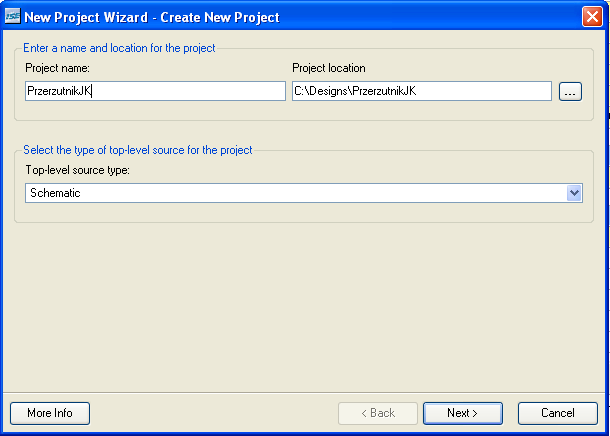
\includegraphics[width=0.7\linewidth]{1.PNG}}\\
\centerline{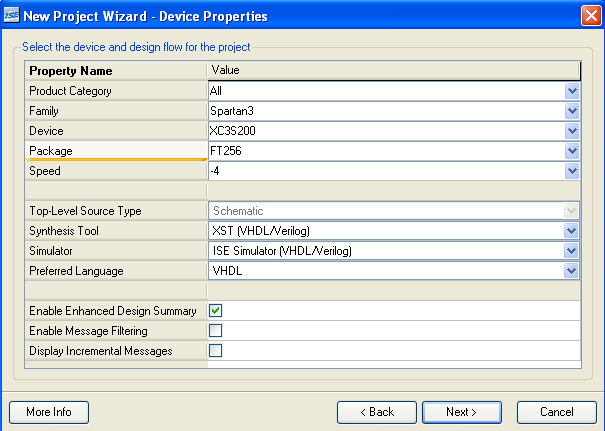
\includegraphics[width=0.7\linewidth]{2.PNG}}\\
Nacisnąć przycisk Next. Następnie nacisnąć Add Source i wybrać pliki:\textit{ jk\_flip\_flop.sch} oraz \textit{board.ucf} z pobranego wczesniej folderu. Następnie nacisnąć kolejne przyciski Next i Finish.
\item Następnie należy utworzyć plik symulacyjny testbench, dzięki czemu będzie można przetestować zaprojektowany układ przed zaprogramowaniem urządzenia docelowego. Aby to uczynić należy w okienku Sources kliknąć prawym przyciskiem myszy na pliku schematu \textit{jk\_flip\_flop.sch} i wybrać opcję New Source. W wyświetlonym oknie wybrać opcję \textit{Test Bench Waveform} i nadać nazwę pliku. Następnie nacisnąć dwukrotnie przycisk Next oraz na koniec Finish. Pojawi się kolejne okienko w którym należy wydłużyć czas trwania symulacji do 4 $\mu$s (parametr Initial Length w prawym dolnym rogu). Ułatwi to zaobserwowanie działania układu. Zamknąć okno przyciskiem Finish. \\
\centerline{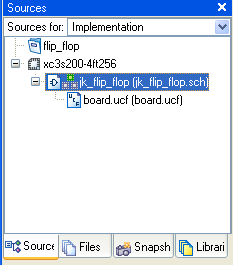
\includegraphics[width=0.29\linewidth]{1_1.PNG}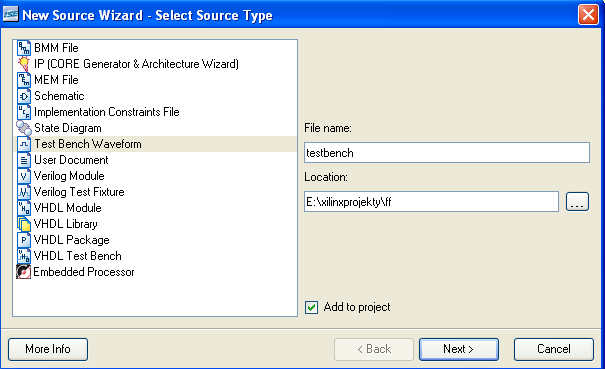
\includegraphics[width=0.69\linewidth]{4.PNG}}
\item We wyświetlonym pliku można dowolnie ustawić sygnały J oraz K, odpowiednio button[0] i button[1]. Sygnał button[2] pełni rolę asynchronicznego resetu. Sygnał zmienia się poprzez naciśnięcie na wykresie czasowym w miejscu w którym chcemy aby nastąpiła zmiana.
\\\centerline{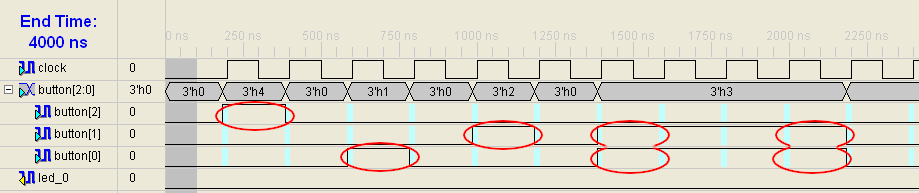
\includegraphics[width=0.8\linewidth]{1_2.PNG}} \\
Na powyższym rysunku zaznaczono przykładowe miejsca kliknięć. Plik zapisać (Ctrl+S).
\item Aby uruchomić symulację należy w oknie Sources wybrać opcję Behavioral Simulation, zaznaczyć utworzony plik *.tbw oraz dwukrotnie kliknąć na pozycji "Simulate Behavioral Model" w oknie Processes.
\\\centerline{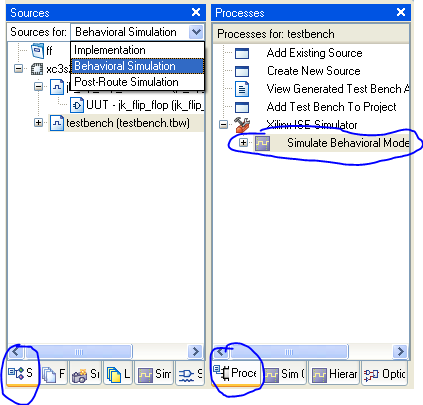
\includegraphics[width=0.8\linewidth]{6.PNG}} \\
\item Jeżeli wyniki symulacji zgadzają się z oczekiwaniami można przejść do testowania układu bezpośrednio na płytce. Aby to zrobić w okienku Sources należy wybrać opcję Implentation i zaznaczyć plik \textit{jk\_flip\_flop.sch}. W okienku Processes należy dwukrotnie nacisnąć Configure Target Device.
\\\centerline{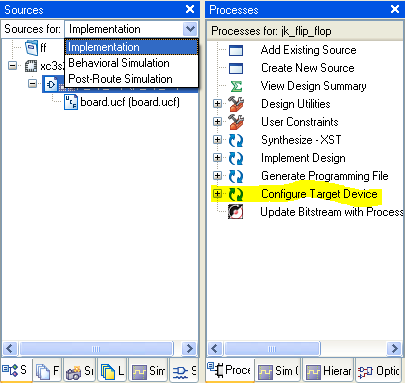
\includegraphics[width=0.5\linewidth]{7.PNG}} \\
Zatwierdzić wywietlony komunikat przyciskiem Ok, a następnie nacisnąć przycisk Finish. W wyświetlonym oknie należy wybrać plik z rozszerzeniem .bit i nacisnąć przycisk Open, a w kolejnym nacisnąć Bypass. W okienku które wyskoczy naciskamy przycisk Ok. Ostatnim krokiem jest naciśnięcie prawym przyciskiem w miejscu jak na rysunku oraz wybrać opcję Program.
\\\centerline{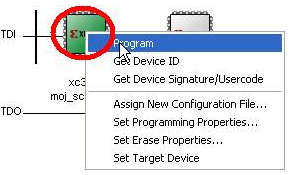
\includegraphics[width=0.5\linewidth]{8.PNG}} \\
\item Można zaobserwować świecenenie diody poprzez naciskanie rożnych kombinacji przycisków, zgodnie z tablicą prawdy przerzutnika JK.
\end{enumerate}
\section{Dzielnik częstotliwości}
W tym zadaniu poruszony zostanie temat dzielnika częstotliwości i do zbadania jego działania zostanie użyta zwykła dioda. Częstotliwość generowana przez kryształ na płytce rozwojowej to 50~MHz, co oznacza, że dioda migałaby co około $2 \cdot 10^{-8}$s, co oczywiście jest niezauważalne dla człowieka. Poprzez zastosowanie układu jakim jest dzielnik częstotliwości, można wydłużyć okres przełączania do np. 1~s. Układ ten zlicza odpowiednią liczbę taktów zegara wejściowego i po przekroczeniu określonej wartości zmienia wartość sygnału na wyjściu, dzięki czemu uzyskujemy odpowiednio ,,spowolniony'' sygnał prostąkątny. W układzie przedstawionym na zajęciach oprócz wejścia i wyjścia występuje przycisk reset, który działa on asynchronicznie, czyli wartość na wyjściu układu zostanie wyzerowana w momencie naciśnięcia przycisku, niezależnie od aktualnego stanu wejściowego sygnału zegarowego.
\subsection{Do wykonania}
\begin{enumerate}[wide, labelwidth=!, labelindent=0pt]
\item Utworzyć nowy projekt wraz z odpowiednimi plikami źródłowymi.
\item Przeanalizować schemat układu. W jaki sposób można zmienić wartość dzielnika?
\item Wgrać program do systemu docelowego.
\end{enumerate}
\subsection{Krok po kroku}
\begin{enumerate}[wide, labelwidth=!, labelindent=0pt]
\item Zamknąć poprzedni projekt (File > Close project).
\item Utworzyć projekt i dodać do niego pliki z folderu \textit{blinking\_led}, czyli \textit{blinking\_led.sch}, \textit{board.ucf}, \textit{frequency\_divider.sym} oraz \textit{frequency\_divider.vhd}, w podobny sposób, jak do poprzedniego zadania (podpunkt 1.2.3.).
\item W celu zmiany wartości dzielnika należy uruchomić w oknie \textit{Sources} dwukrotnie kliknąć plik \textit{blinking\_led.sch}.\\
\centerline{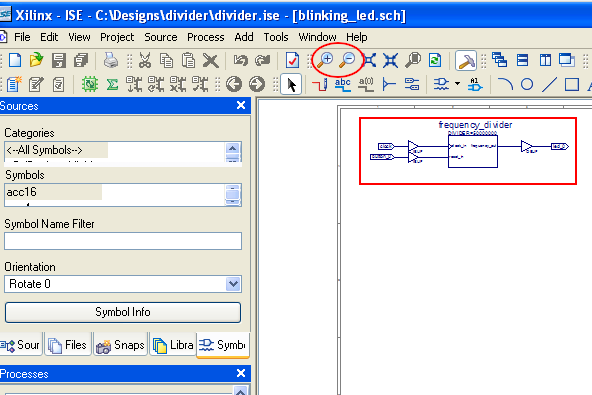
\includegraphics[width=0.5\linewidth]{2_1.png}}
\item Przybliżyć schemat tak aby widoczne były jego wszystkie elementy, następnie kliknąć prawym przyciskiem myszy na bloku dzielnika i wybrać pozycję \textit{Object Properties}.\\
\centerline{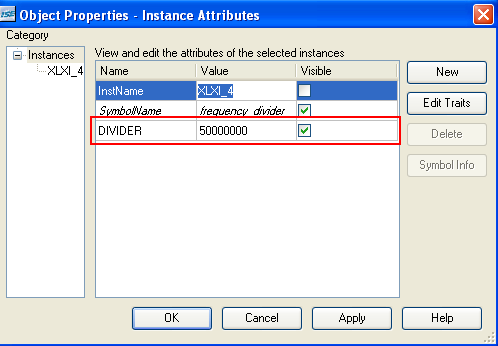
\includegraphics[width=0.5\linewidth]{2_2.png}}
\item Zmienić wartość dzielnika (pole DIVIDER). Domyślna wartość $5\cdot 10^{7}$ odpowiada częstotliwości wyjściowej 1 Hz.
\item Aby zaprogramować układ w systemie docelowym należy postąpić podobnie jak w poprzednim ćwiczeniu (podpunkt 1.2.7.).
\end{enumerate}
\section{Sterownik wyświetlacza siedmiosegmentowego}
Kolejnym układem którego działanie zostanie zaprezentowane jest wyświetlacz siedmiosegmentowy. Taki wyświetlacz, dzięki swojej prostocie, powszechnie używany jest do wyświetlania liczb. Pojedynczy wyświetlacz składa się z siedmiu segmentów, które zostają podświetlane zależnie od danych jakie chcemy wyświetlić.\\
\centerline{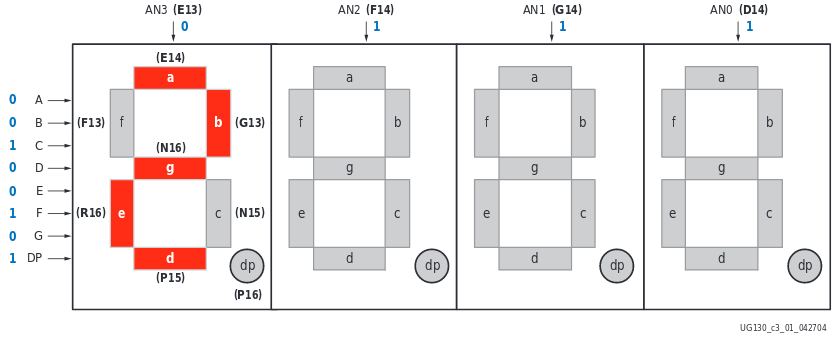
\includegraphics[width=1\linewidth]{3_1.png}}\\
Na płytce rozwojowej dostepnej w laboratorium występuje poczwórny wyświetlacz, który posiada jedną ośmiobitową linię zapalającą segmenty (zobrazowaną po lewej) oraz cztery linie aktywujące wyświetlanie (widoczne na górze). W konsekwencji jeśli na każdym wyświetlaczu chcemy wyświetlić inny znak (aby przykładowo wyświetlić jakąś liczbę) musimy dokonać multipleksacji, co sprowadza się do sekwencyjnego zapalania każdego z wyświetlaczy. Najpierw ustawiamy dane pierwszego wyświetlacza i go aktywujemy, następnie wyświetlacz ten wygaszamy, zmieniamy dane i zapalamy drugi itd. Aby znak został wyświetlony tylko na jednym wyświetlaczu, na linii aktywującej konkretny wyświetlacz powinna wystąpić wartość 0, a na innych liniach 1 (wejście aktywne stanem niskim). Aby taki układ działał poprawnie, musi działać z odpowiednią częstotliwością. Częstotliwość ta musi być odpowiednio wysoka, aby ludzkie oko nie wychwyciło migotania obrazu, ale też nie za wysoka, aby kolejne wyświetlacze zdążyły się wygasić przed zmianą danych. Na potrzeby tego zadania została przyjęta 1~kHz, więc do tego celu w sterowniku został użyty dzielnik częstotliwości ze zadania poprzedniego.
\subsection{Do wykonania}
\begin{enumerate}[wide, labelwidth=!, labelindent=0pt]
\item Utworzyć nowy projekt. Pobrać ze strony folder \textit{display\_controler\_test}. Do projektu dodać następujące pliki: \textit{OBUF4\_magistral.sch}, \textit{OBUF4\_magistral.sym}, \textit{board.ucf},\\ \textit{display\_controler\_test.sch}, \textit{display\_led7seg\_controler.sym}, \textit{display\_led7seg\_controller.vhd}, \textit{frequency\_divider.sym}, \textit{frequency\_divider.vhd}.
\item Przeanalizować schemat wyświetlacza. W jaki sposób zapamiętywane są wyświetlane znaki?
\item Wgrać program do systemu docelowego. Jaka jest największa liczba możliwa do wyświetlenia?
\end{enumerate}
\section{Stoper}
Ostatnim przewidzianym na zajęcia zadaniem jest zbadanie praktycznego wykorzystania wszystkich poprzednich układów. Stoper składa się on ze sterownika wyświetlania, czterech liczników modulo 10 połączonych kaskadowo oraz dzielnika częstoliwości wykorzystanego w celu uzyskania stałej częstotliwości 100~Hz. Częstotliwość ustala rozdzielczość pomiaru czasu na poziomie 10~ms.
\subsection{Do wykonania}
\begin{enumerate}[wide, labelwidth=!, labelindent=0pt]
\item Utworzyć nowy projekt. Pobrać ze strony folder \textit{stopwatch}. Do projektu dodać następujące pliki: \textit{OBUF4\_magistral.sch}, \textit{OBUF4\_magistral.sym}, \textit{board.ucf}, \textit{counter\_modulo\_10.sym}, \textit{counter\_modulo\_10.vhd}, \textit{display\_led7seg\_controler.sym}, \textit{display\_led7seg\_controller.vhd},\\ \textit{frequency\_divider.sym}, \textit{frequency\_divider.vhd}, \textit{stopwatch.sch}.
\item Przeanalizować schemat stopera. Jakie są funkcje poszczególnych przycisków?
\item Wgrać program do systemu docelowego. Co się dzieje, gdy mierzony czas przekracza 99,99~s?
\end{enumerate}
\end{document}
